\documentclass[12pt, a4paper]{article}

\usepackage[utf8]{inputenc}
\usepackage[english, ngerman]{babel}
\usepackage{graphicx}

\title{Summary Image Processing}
\author{Abderrahmen Rakez}
\date{}

\begin{document}
\maketitle

\section{course goals}
\begin{itemize}
  \item[*] introduction to the fundamentals of rasterization-based image generation: rasterization is the task of taking an image described in a vector graphics format and converting it into
  a raster image(pixels or dots) for output on a video display or printer, or for storage in a bitmap file format.
  \item[*] functionality of the graphics rendering pipline: Rendering is the automatic porcess of generating a photorealistic or non-photorealistic image
  from a 2D or 3D model by means of computer graph
  \item[*] advanced rendering effects
  \item[*] introduction to the openGL graphics API
\end{itemize}

\section{OpenGL}
\subsection{Intoduction}
OpenGL (Open Graphics Library) is a cross-plarform API\footnote{Application Programming Interface} for rendering 2D and 3D vertor graphics\footnote{is the use of polygons(are used in Com.
Graphics to compose images that are 3-dim in appearence) to represent images in computer graphics}...
\begin{itemize}
  \item[*] display of geometric representations and attributes
  \item[*] independent from operating system and window system
\end{itemize}

\subsection{GPU Data Flow}
\begin{itemize}
  \item[*] data tramsfer to GPU: vertices with attribures and connectivity
  \item[*] vertex shader\footnote{are HW or SW modules, that implement spezific redering}: a program that is executed for each vertex, with input and output is a vertex
  \item[*] rasterizer
  \item[*] fragment shader: also known pixel shader, a program that is executed for each fragement, with input and output is a fragment. compute color and other attribures of each fragment\footnote{
  a technical term usally meaning a single pixel }
  \item[*] framebuffer update: is portion of RAM containing a bitmap that drives a video display. It is a memory buffer containing a complete frame of data
\end{itemize}

\section{Rendering}
\subsection{Rasterization}
\begin{itemize}
  \item[*] rendering algorithm for generating 2D images form 3D scenes
  \item[*] transforming geometric primitives such as lines and polygons into raster image representations, i.e pixels
  \item[*] 3D objects are approximitely represented by vetices(points), lines, polygons
  \item[*] these primitives are processed to obtain a 2D image
\end{itemize}

\subsection{Redenting Pipeline}
known also as graphics pipeline is a concenptual model in computer graphics that describe what step a graphics system needs to perform to render a 3D scene to a 2D screen, plainly speaking, the
graphics pipeline is the process of turning that 3D model into what the computer displays. \\
Characteristics of the 3D input:
\begin{enumerate}
  \item a virtual camera: positon, orientation, focal lenght
  \item objects: points(vertex/vertices), lines, polygons, geometry and merial properties
  \item light sources: direction, postion, color, intensity
  \item textures(images)
\end{enumerate}
Characteristics of the 2D output: per-pixel color value in the framebuffer

\section{Transformations}
\begin{itemize}
  \item[*]  is used to: position, reshape, and animate objects, lights, and the virtual camera
  \item[*]  are respresented with 4x4 matrices
  \item[*]  are applied to vertices and normals
  \item[*]  vertices(position) and normals(directions) are represented with 4D vectors
\end{itemize}

\subsection{Modelview Transform}
\begin{figure}[!ht]
  \centering
  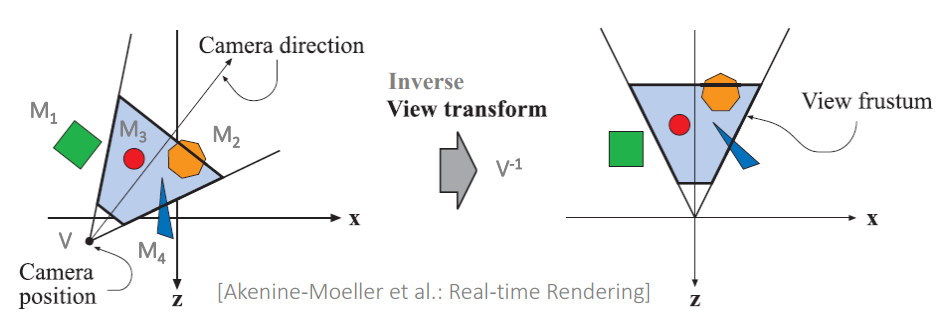
\includegraphics[width=\textwidth]{image/viewTransform}
  \label{}
\end{figure}

\begin{itemize}
  \item[*] M$_{1..4}$ and V are matrices representing transformations
  \item[*] M$_{1..4}$ are model transform to place the objects in the scene
  \item[*] V places and orientates the camera in space, V$^-1$ transforms the camera to the origin looking along the negative z-axis
  \item[*] model and view transforms are combined in the modelview transform
  \item[*] the modelview tranform V$^-1$M$_{1..4}$ is applied to the objects
\end{itemize}

\subsection{Prjection Trasform}
\begin{itemize}
  \item[*] P transforms the view volume to the canonical view volume
  \item[*] the view volume depends on the camera properties : \begin{enumerate}
    \item orthographic projection $==>$ cuboid
    \item perspective projection $==>$ pyramidal frustum
  \end{enumerate}
  \item[*] canonical view volume is a cube from (-1, -1, -1) to (1, 1, 1)
  \item[*] view volume is specified by near, far, left, right, bottom, top
\end{itemize}
\begin{figure}[!ht]
  \centering
  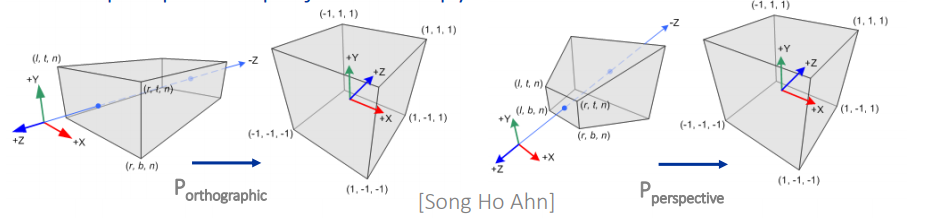
\includegraphics[width=\textwidth]{image/projectionTrasform}
  \label{}
\end{figure}

\subsection{Viewport Transform / Screen Mapping}
\begin{itemize}
  \item[*] prjected primitive coordinates (x$_p$, y$_p$, z$_p$) are transformed to screen coordinates (x$_s$, y$_s$)
  \item[*] screen coordinates together with depth value are window coordinates (x$_s$, y$_s$, z$_w$)
\end{itemize}

\begin{figure}[!ht]
  \centering
  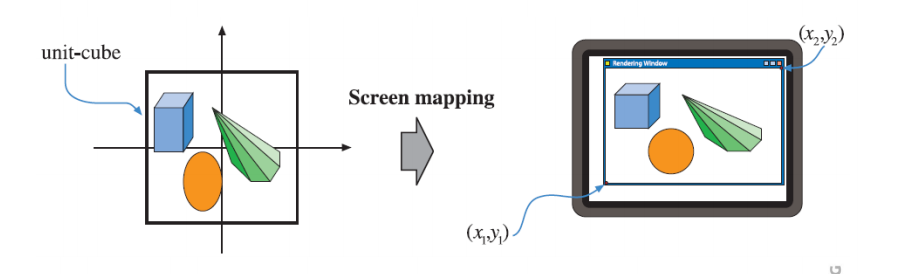
\includegraphics[width=\textwidth]{image/viewportTransform}
  \label{}
\end{figure}

\subsection{Vertex Transforms}
Vertex is a data structure that describes certain attribute, like the position of a point in 2D or 3D space ... \\
the vertex tranform went through some transformation before achieving the window space, like model trans., inverse view trans., projection trans., and viewport trans.

\subsection{Other Transformation}
\begin{itemize}
  \item[*] congurent transformations (Euclidean transformations)
  \item preserve shape and size
  \item translation, rotation, reflection
  \item[*] similarity transformations
  \item preseve shape
  \item translation, rotation, reflection, scale

\subsection{Affine Transformations}
Folie Seite 12.

\section{Lighting}
\subsection{Light}
Light is modeled as: \begin{itemize}
  \item electromagnetic waves
  \item photons: are particles characterized by wavelength, which carry energy. They travel along a straight line at the speed of light
  \item geometric rays
\end{itemize}
the discipline of optical measurement techniques can be roughly subdivided into the two area of \textbf{photometry} and \textbf{radiometry}

\subsubsection{Radiometric Quantities}
Radiometry deals with the measurement of energy per time also \textbf{Power}
\begin{itemize}
  \item radiant energy Q: photons have some radiant energy
  \item radiant flux $\Phi$, radiant power P: the rate of flow of radiant energy per unit time is defined as follow: $\Phi$ $=$ $\frac{d Q}{d t}$, for example the overall energy of photons emitted by a source per time
  \item flux density: is the radiant flux per unit area: E $=$ $\frac{d \Phi}{d A}$, which is the rate at which radiation is incident on, or exiting a flat surface area dA, it discribes also the strength of radiation with respect to a surface area with no directional information
\end{itemize}





\end{itemize}


\end{document}
